\section{Literature Review}
There are various approaches to perform segmentations of images. While the traditional methods like thresholds or edge detection are based on deterministic algorithms, more recent experiments make use of probabilistic techniques. This chapter addresses the basics and recent development of Deep Learning methods in detail and highlights the most important architectural patterns.

\subsection{Deep Learning Basics}
\emph{Deep Learning} is a new field of machine learning that makes use of \emph{Deep Neural Networks} (DNN)~\cite[pp.~125f]{nn_intro96}. In an abstract point of view, a DNN is just a mathematical function to map a given input vector to an output vector. It is assembled from densely-connected units called \emph{neurons} (or \emph{perceptrons}).

Usually, the neurons are grouped into layers~\cite[p.~125]{nn_intro96} (see figure~\ref{fig:layered_architecture}). The first layer of the DNN has direct access to the input vector, thus it is called the \emph{input layer}. In contrast, the last layer of the DNN produces the output vector and is therefore called \emph{output layer}. In between, there is an arbitrary number of \emph{hidden layers} that make up for the depth of the neural network.

\begin{figure}[h]
    \centering
    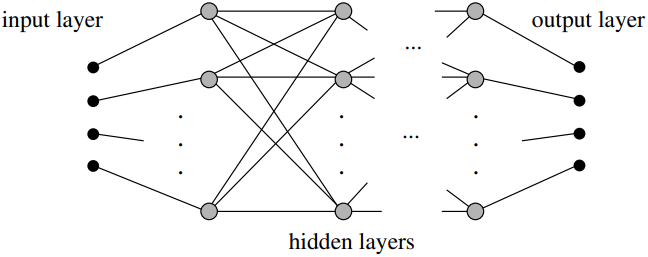
\includegraphics[width=0.7\textwidth]{images/generic_layered_architecture}
    \caption[A Generic Layered DNN Architecture]{A Generic Layered DNN Architecture~\cite[p.~126]{nn_intro96}}
    \label{fig:layered_architecture}
\end{figure}

Each neuron is itself a small computational unit that applies several mathematical operations, namely an \emph{input function} and an \emph{activation function}. Traditionally, the neurons of subsequent layers are densely connected, meaning a neuron of layer $k$ receives the output values from all neurons in layer $k-1$. Based on those values, the input function calculates the \emph{net input} for the neuron. In most cases this is done by using weights on the connections to perform a weighted sum over all values.

The net input is then passed through the activation function whose main purpose is to break the linearity of the DNN. For the activation function there are plenty of options to choose from. An overview of commonly used activation functions can be found in~\cite{act_funcs18} and includes for example a binary step function, a sigmoid function or rectified linear units (ReLU). Some activation functions require a threshold value to control the sensitivity of the neuron. Figure~\ref{fig:perceptron} depicts all the calculations done inside of a neuron.

\begin{figure}[h]
    \centering
    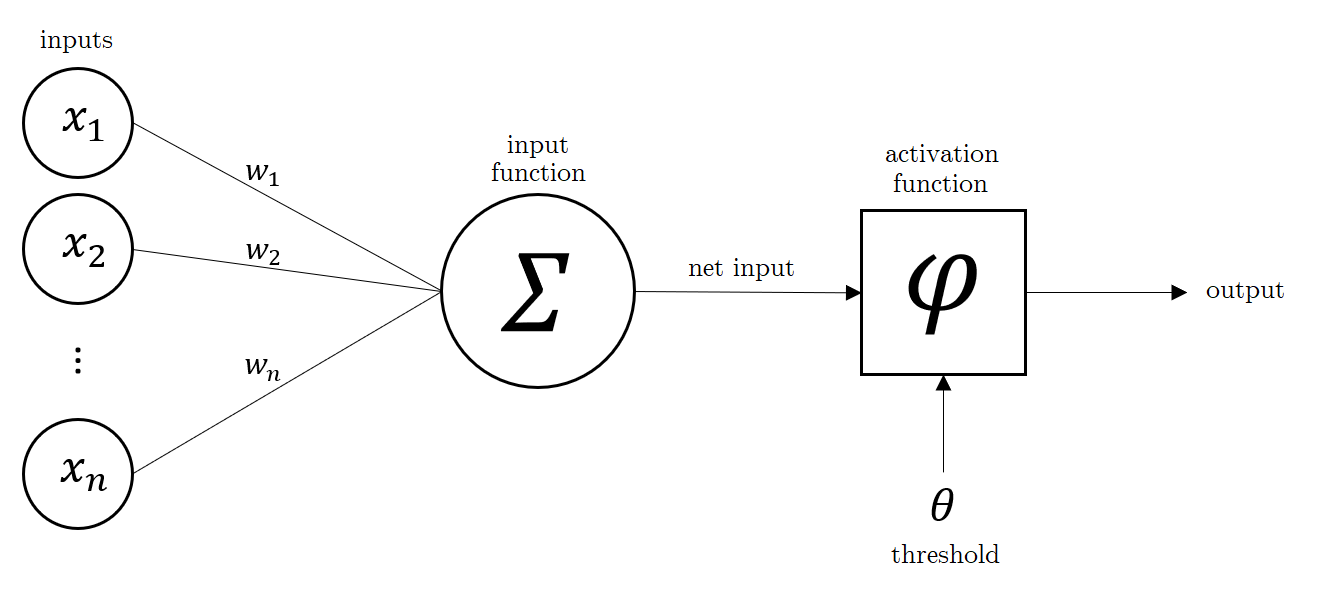
\includegraphics[width=0.7\textwidth]{images/perceptron}
    \caption[Schematic View of a Perceptron]{Schematic View of a Perceptron~\cite[p.~257, modified]{praxiseinstieg_ml17}}
    \label{fig:perceptron}
\end{figure}

To adapt a DNN model for a specific task, the weights for all the connections have to be initialized with proper values. Since there are so many weights, it is not feasible to choose the values by hand, but rather use a process called \emph{training}. To train the DNN model, it is fed with examples of input vectors with their respective output vectors. During this process the weights are adjusted slightly, so that the model better reflects the relations between the input and the output vectors. This is a computationally intensive process that requires a large amount of training data. After repeating this with thousands of training vectors, the weights of the model will eventually converge to fit the task.

\subsubsection{Training with Backpropagation}
One of the most commonly used algorithms to perform the training is the \emph{backpropagation algorithm}~\cite[pp.~151ff]{nn_intro96}. It relies on an \emph{error function} (sometimes also called \emph{loss function}), which is meant to calculate the deviation between the model's current output vector and the desired output vector. The backpropagation algorithm then searches for a minimum of the error function by adjusting the model's weights according to an \emph{optimization strategy}. Which algorithms to choose for both the error function and the optimization strategy is highly dependent on the task to solve and on the quality requirements for the final predictions.

The concept of backpropagation is to do a standard forward pass through the model with one batch of data to calculate the output vector and the activations from all the neurons. After that, the predicted output vector is compared to the desired output vector using the error function to get the total error. Based on the total error and the activations of the neurons, the backpropagation algorithm now determines the effect each single neuron contributes to the total error rate. In the end, the weights are adjusted in such a way, that the total error rate is likely to decrease.

Sometimes it can happen that the total error increases after the weights are adjusted. This is because the backpropagation algorithm only indicates the direction (positive or negative) in which each weight should be moved. But it can not predict the order of magnitude for the adjustment. For that, a parameter called \emph{step width} (often referred to as \emph{learning rate}) is introduced~\cite[p.~169]{nn_intro96}. If the learning rate is too big, it can happen that the adjusted weights overshoot the minimum of the error function, resulting in an increased error rate. On the other hand, if the learning rate is too small, the training requires even more iterations. Therefore, it is very important to pick an appropriate learning rate for the model.

\subsubsection{Optimizing the Training Algorithm}
DNNs are very flexible and allow to solve a broad variety of tasks. However, this flexibility also comes with some challenges. For example, DNNs include countless configuration options, all of which affect the final outcome. Those options are commonly referred to as \emph{hyperparameters}~\cite[pp.~270ff]{praxiseinstieg_ml17}. 

In general, a hyperparameter is an option of the learning algorithm. It is not learned during training, but rather set beforehand. Hyperparameters cover all kinds of options, such as loss and activation functions. Also the overall architecture of the model can be seen as a hyperparameter. This includes for example the number of layers, number of neurons per layer and much more.

A major challenge in building deep learning models is to optimize the hyperparameters for the specific task. Since often the training of a single model is already very time consuming, it is not feasible to explore all permutations of hyperparameters. There are some strategies to deal with this issue. Two popular approaches are \emph{grid search} and \emph{random search}~\cite[pp.~73ff]{praxiseinstieg_ml17}.

For the grid search some options for the hyperparameters have to be  picked manually. The search then computes the results of all permutations of the given parameters. This means, for each permutation a model is built, trained and evaluated. This strategy yields a good overview over the optimization potential. However, it can be very time consuming and expensive depending on the number of combinations. Thus, it is not applicable for every case.

If there are too many combinations, a random search can be consulted instead. Basically it works in the same way. However, not all permutations are evaluated but only a few random samples. This speeds up the search process significantly, but the results are less informative. Usually, a random search still reveals some optimization patterns in the hyperparameters that can be further explored.

\subsubsection{Common Paradigms for Deep Learning}
\label{sec:dl_paradigms}
In general, there are three major paradigms to categorize DNNs based on their learning behaviour~\cite[p.~214f]{dlma14}. First, \emph{supervised learning} improves the network by using predefined pairs of input and output during the training period. This means during training, the expected output (also called \emph{label} or \emph{ground truth}) is directly exposed to the network. Supervised learning fits great for classification tasks, because it allows to guide the discriminative power of the network with the provided labels. In most cases, it needs lots of labelled data to learn from. The preparation of the labels usually involves a high level of manual work. The architectures presented in sections~\ref{sec:unet} and~\ref{sec:densenet} make use of this learning method.

\emph{Unsupervised learning} does not need any labels for the training process. It is commonly used for tasks like representation learning, trying to compress the input data in a more compact format with only minimal loss in information. Generally speaking, the purpose of unsupervised learning is to find correlations in the dataset, that help forming a deeper understanding of the data. It can also be used to perform unsupervised information clustering or segmentation, as discussed later in section~\ref{sec:w-net}.

The last category is called \emph{reinforcement learning} and is suited for tasks that require interaction with the environment. Based on the actions the network takes, it is either rewarded or punished. For the purpose of this thesis reinforcement learning will not be further explored.

\subsection{Computer Vision Tasks}
There are many different tasks in computer vision for detecting and labelling objects in images. This section will give a brief summary of common tasks in the field. In addition, popular datasets with their scoring methods and suitable approaches to solving the problems are presented.

One of the easier tasks is called \emph{image classification}~\cite[p.~98]{DLbook16}. It is about choosing a matching class from a set of predetermined classes for a single image (see figure~\ref{fig:cv_task_imgclass}). To achieve that, recent approaches use convolutional neural networks as described in section~\ref{sec:cnn}. The output is a probability distribution which indicates the likelihood that the image will fit into a class. The class with the highest probability score can then be selected as the final prediction for the image. A popular dataset for this task is the \emph{MNIST handwritten digits database}~\cite{mnist10}. To measure the performance of the solutions, the challenge recommends to compare the relative error rate of wrong class predictions in the test set.

The next level is to not only assign a label to an image, but also detect where the object in the image is located (see figure~\ref{fig:cv_task_objloc}). Thus, this task is referred to as \emph{object localization}~\cite{rcnn14}. In addition to the class label, the output is extended by a rectangular bounding box that encloses the spatial extent of the object. This change allows to detect multiple objects in the same image, each with a class label and a (possibly overlapping) bounding box. There are different ways to solve this task, like for example bounding box regression~\cite{obj_detection13} or region proposal networks~\cite{ff-rcnn14}. The \emph{ImageNet} dataset presented in~\cite{imgnet09} provides millions of images with prepared object classes and bounding boxes. The performance measurement for this dataset is calculated by matching the predicted objects for an image and evaluating the overlapping area in the bounding boxes.

\begin{figure}
    \newcommand{\VisionTasksImageWidth}{0.4\textwidth}
    \centering
    \begin{subfigure}{\VisionTasksImageWidth}
        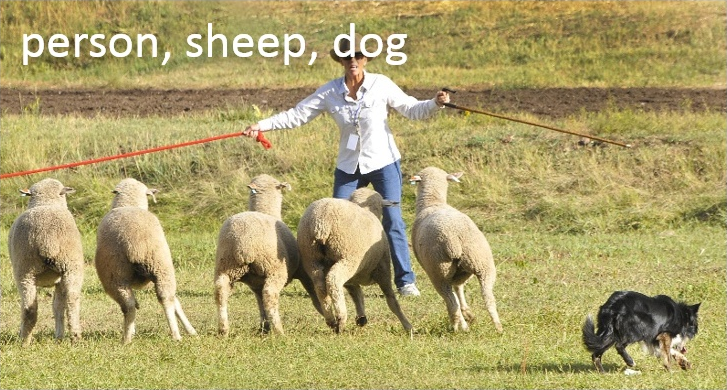
\includegraphics[width=\textwidth]{images/vision_task_1}
        \caption{Image Classification}
        \label{fig:cv_task_imgclass}
    \end{subfigure}
    \hspace{5mm}
    \begin{subfigure}{\VisionTasksImageWidth}
        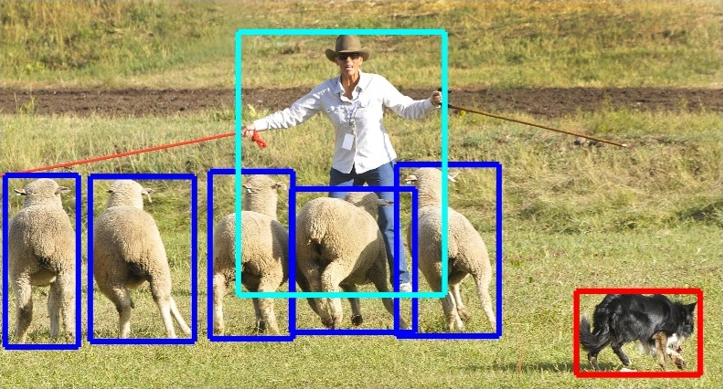
\includegraphics[width=\textwidth]{images/vision_task_2}
        \caption{Object Localization}
        \label{fig:cv_task_objloc}
    \end{subfigure}

    \vspace{5mm}
    
    \begin{subfigure}{\VisionTasksImageWidth}
        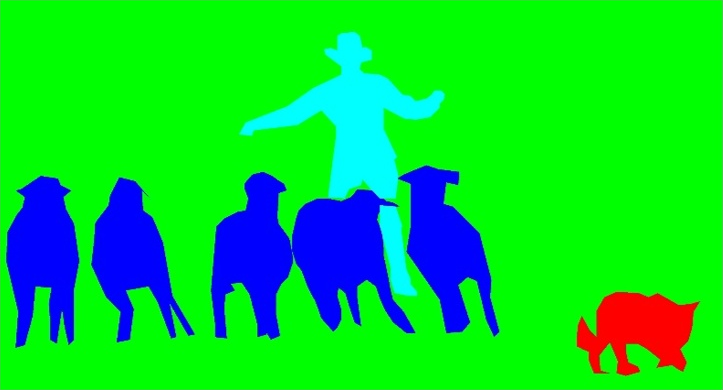
\includegraphics[width=\textwidth]{images/vision_task_3}
        \caption{Semantic Segmentation}
        \label{fig:cv_task_semseg}
    \end{subfigure}
    \hspace{5mm}
    \begin{subfigure}{\VisionTasksImageWidth}
        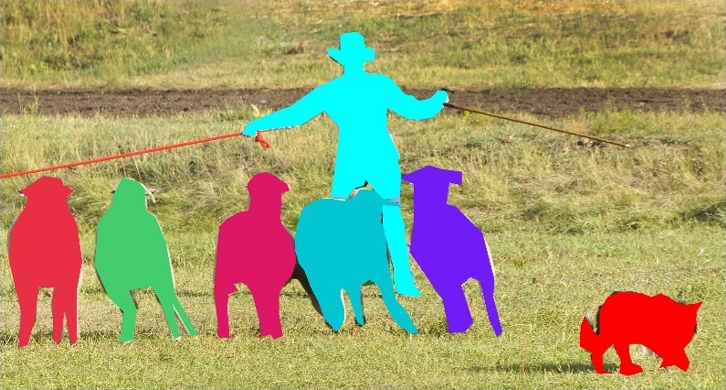
\includegraphics[width=\textwidth]{images/vision_task_4}
        \caption{Instance Segmentation}
        \label{fig:cv_task_inseg}
    \end{subfigure}

    \caption[Computer Vision Tasks]{Computer Vision Tasks~\cite{coco15}}
    \label{fig:cv_tasks}
\end{figure}

Rectangular boxes are not very accurate for expressing the spatial extents of an object. Therefore, another task called \emph{semantic segmentation}~\cite{weakseg15} deals with pixel-level classification of an image (see figure~\ref{fig:cv_task_semseg}). This determines a precise mask telling for each pixel of the image the object it belongs to. Since this is one of the main tasks of this thesis, an in-depth discussion of modern solutions to this task follows in section~\ref{sec:ref_archs}. One dataset to measure the performance of the various approaches is the Pascal Visual Object Classes as laid out in~\cite{pascal_voc15}. The scoring is done by calculating the \emph{intersection over union} (IoU) metric, which is explained in detail in section~\ref{sec:metrics}.

The last task to mention here is called \emph{instance segmentation}~\cite{mask-rcnn14}. Whereas previously only one class had to be assigned to each pixel, a distinction is now also made between pixels that belong to the same object class but different instances of an object (see figure~\ref{fig:cv_task_inseg}). This task is quite challenging, as for example parts of an instance can be hidden by another instance of the same class, which leads to gaps in the mask. \emph{Mask R-CNN}~\cite{mask-rcnn14} is a widely used meta-algorithm for solving this task. It combines region proposals used for object localization with semantic segmentation processes. A great dataset for this challenge is the \emph{Microsoft Common Objects in Context} set, which can be found in~\cite{coco15}.

\subsection{Convolutional Neural Networks}
\label{sec:cnn}

One subclass of neural networks is called \emph{Convolutional Neural Network} (CNN)~\cite[p.~359]{praxiseinstieg_ml17}. These types of networks show great results on data with a grid-like topology. Thus, they are often used for processing image or video data that essentially consists of a grid of colored pixels.

Traditionally, the layers in DNNs are densely connected, meaning every neuron of one layer is connected to every neuron in the next layer. For grid-like data this is not very efficient, because cells close to each other are often more likely to be correlated. Although this relationship is also represented in densely-connected architectures, it requires a lot of computational power to learn the exact spatial correlations. Hence it is better to embed the spatial concept directly into the architectural design of the network.

Instead of dense connections, CNNs use operations called \emph{convolution} and \emph{pooling}, which allow to take spatial properties of the input data into account. The following sections explain those commonly used operations in CNNs.

\subsubsection{Convolution}
\label{sec:convolution}
\emph{Convolution} is a mathematical operation that uses weighted point-by-point multiplication of two matrices resulting in a scalar value~\cite[p.~361 f]{praxiseinstieg_ml17}. It involves a multiplication kernel which is moved pixel by pixel across the image. In each step the kernel computes an output value for a small part of the image (called \emph{receptive field}). Depending on the values in the kernel, this technique highlights certain features in the image like edge orientation, colors and gradients. The outcome of a convolution operation is a convoluted image, which represents a heatmap for one specific feature with respect to the input image. The concept is shown in figure~\ref{fig:convolution}.

\begin{figure}[h]
    \centering
    \definecolor{conv_lightgreen}{HTML}{bdddbd}
\definecolor{conv_darkgreen}{HTML}{8dbd8d}
\definecolor{conv_lightred}{HTML}{cdcddd}
\definecolor{conv_darkred}{HTML}{9d9dbd}

\newcommand{\filtersize}{3}
\newcommand{\filterx}{8}
\newcommand{\filtery}{2.2}
\newcommand{\filteroffset}{1}

\newcommand{\filterxres}{12}

\newcommand{\imagesize}{7}
\newcommand{\imagex}{0}
\newcommand{\imagey}{0}
\newcommand{\imageoffset}{2}

\newcommand{\outx}{12}
\newcommand{\outy}{0}
\newcommand{\outoffset}{2}

\newcommand{\percx}{1}
\newcommand{\percy}{2}
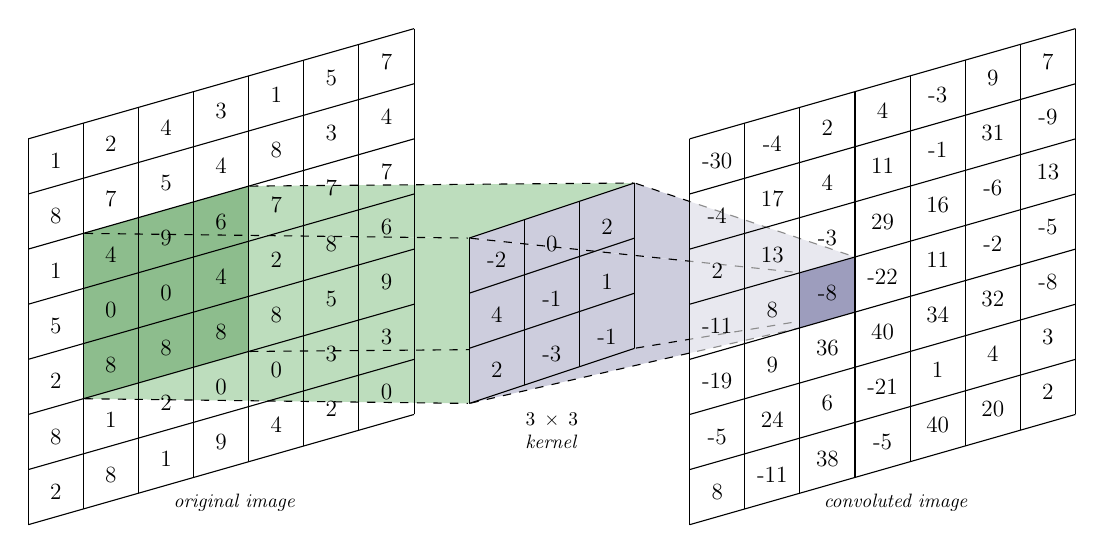
\begin{tikzpicture}[scale=0.7, every node/.style={transform shape}]
    \tikzstyle{point}=[draw=none,inner sep=0pt]

    % corner points of perceptive field
    \node (p1)[point] at (\imagex+\percx, \imagey+\percy+\percx*\imageoffset/\imagesize) {};
    \node (p2)[point] at (\imagex+\percx+\filtersize, \imagey+\percy+\percx*\imageoffset/\imagesize+\filtersize*\imageoffset/\imagesize) {};
    \node (p3)[point] at (\imagex+\percx+\filtersize, \imagey+\percy+\filtersize+\percx*\imageoffset/\imagesize+\filtersize*\imageoffset/\imagesize) {};
    \node (p4)[point] at (\imagex+\percx, \imagey+\percy+\filtersize+\percx*\imageoffset/\imagesize) {};

    % corner points of filter
    \node (f1)[point] at (\filterx, \filtery) {};
    \node (f2)[point] at (\filterx+3, \filtery+1) {};
    \node (f3)[point] at (\filterx+3, \filtery+4) {};
    \node (f4)[point] at (\filterx, \filtery+3) {};

    % corner points of output point
    \node (o1)[point] at (\outx+\percx+1, \outy+\percy+\percx*\outoffset/\imagesize+1+1*\outoffset/\imagesize) {};
    \node (o2)[point] at (\outx+\percx+2, \outy+\percy+\percx*\outoffset/\imagesize+1*\outoffset/\imagesize+1+1*\outoffset/\imagesize) {};
    \node (o3)[point] at (\outx+\percx+2, \outy+\percy+1+\percx*\outoffset/\imagesize+1*\outoffset/\imagesize+1+1*\outoffset/\imagesize) {};
    \node (o4)[point] at (\outx+\percx+1, \outy+\percy+2+\percx*\outoffset/\imagesize+1*\outoffset/\imagesize) {};

    % corner points of output image
    \node (op1)[point] at (\outx, \outy) {};
    \node (op2)[point] at (\outx+\imagesize, \outy+\outoffset) {};
    \node (op3)[point] at (\outx+\imagesize, \outy+\imagesize+\outoffset) {};
    \node (op4)[point] at (\outx, \outy+\imagesize) {};

    % draw image to filter shadow
    \fill[conv_lightgreen] (p1.center) -- (f1.center) -- (f4.center) -- (p4.center) -- (p1.center);
    \fill[conv_lightgreen] (f4.center) -- (f3.center) -- (p3.center) -- (p4.center) -- (f4.center);

    % draw perceptive field
    \fill[conv_darkgreen] (p1.center) -- (p2.center) -- (p3.center) -- (p4.center) -- (p1.center);

    % draw dashed connections image to filter
    \draw[dashed] (p1) -- (f1);
    \draw[dashed] (p2) -- (f2);
    \draw[dashed] (p3) -- (f3);
    \draw[dashed] (p4) -- (f4);

    % hide dashed lines behind filter
    \fill[white] (f1.center) -- (f2.center) -- (f3.center) -- (f4.center) -- (f1.center);

    % filter to output point
    \fill[conv_lightred] (f1.center) -- (o1.center) -- (o4.center) -- (f4.center) -- (f1.center);
    \fill[conv_lightred] (f4.center) -- (o4.center) -- (o3.center) -- (f3.center) -- (f4.center);

    % draw dashed connections filter to out
    \draw[dashed] (f1) -- (o1);
    \draw[dashed] (f2) -- (o2);
    \draw[dashed] (f3) -- (o3);
    \draw[dashed] (f4) -- (o4);

    % white overlay for output
    \fill[white, fill opacity=0.55] (op1.center) -- (op2.center) -- (op3.center) -- (op4.center) -- (op1.center);

    % draw output point
    \fill[conv_darkred] (o1.center) -- (o2.center) -- (o3.center) -- (o4.center) -- (o1.center);

    % draw image
    \foreach \x in {0,...,\imagesize}
    {
    \draw (\imagex+\x, \imagey+\x*\imageoffset/\imagesize) -- (\imagex+\x, \imagey+\imagesize+\x*\imageoffset/\imagesize);
    \draw (\imagex, \imagey+\x) -- (\imagex+\imagesize, \imagey+\x+\imageoffset);
    }

    % draw filter
    \foreach \x in {0,...,\filtersize}
    {
    \draw (\filterx+\x, \filtery+\x*\filteroffset/\filtersize) -- (\filterx+\x, \filtery+\filtersize+\x*\filteroffset/\filtersize);
    \draw (\filterx, \filtery+\x) -- (\filterx+\filtersize, \filtery+\x+\filteroffset);
    }

    % draw out
    \foreach \x in {0,...,\imagesize}
    {
    \draw (\outx+\x, \outy+\x*\outoffset/\imagesize) -- (\outx+\x, \outy+\imagesize+\x*\outoffset/\imagesize);
    \draw (\outx, \outy+\x) -- (\outx+\imagesize, \outy+\x+\outoffset);
    }

    \node at (\imagex + \imagesize/2 + 0.25,\imagey+0.4) {\emph{original image}};
     \node[text width=4cm, align=center] at (\filterx + \filtersize/2,\filtery + \filtersize - 3.5) {\emph{$3\times 3$\\kernel}};
    \node at (\outx + \imagesize/2 + 0.25,\outy+0.4) {\emph{convoluted image}};

    % Start image (left to right, top to bottom)
    \node[draw=none] at (0.5, 6.6) {\large 1};
    \node[draw=none] at (1.5, 6.9) {\large 2};
    \node[draw=none] at (2.5, 7.2) {\large 4};
    \node[draw=none] at (3.5, 7.5) {\large 3};
    \node[draw=none] at (4.5, 7.8) {\large  1};
    \node[draw=none] at (5.5, 8.1) {\large  5};
    \node[draw=none] at (6.5, 8.4) {\large  7};%%%%%%%%%%%%%%%%%%%%%%%%%%%%%%%

    \node[draw=none] at (0.5, 5.6) {\large 8};
    \node[draw=none] at (1.5, 5.9) {\large  7};
    \node[draw=none] at (2.5, 6.2) {\large 5};
    \node[draw=none] at (3.5, 6.5) {\large 4};
    \node[draw=none] at (4.5, 6.8) {\large 8};
    \node[draw=none] at (5.5, 7.1) {\large 3};
    \node[draw=none] at (6.5, 7.4) {\large  4};%%%%%%%%%%%%%%%%%%%%%%%%%%%%%%%

    \node[draw=none] at (0.5, 4.6) {\large 1};
    \node[draw=none] at (1.5, 4.9) {\large 4};
    \node[draw=none] at (2.5, 5.2) {\large 9};
    \node[draw=none] at (3.5, 5.5) {\large 6};
    \node[draw=none] at (4.5, 5.8) {\large  7};
    \node[draw=none] at (5.5, 6.1) {\large  7};
    \node[draw=none] at (6.5, 6.4) {\large 7};%%%%%%%%%%%%%%%%%%%%%%%%%%%%%%%

    \node[draw=none] at (0.5, 3.6) {\large 5};
    \node[draw=none] at (1.5, 3.9) {\large  0};
    \node[draw=none] at (2.5, 4.2) {\large 0};
    \node[draw=none] at (3.5, 4.5) {\large  4};
    \node[draw=none] at (4.5, 4.8) {\large 2};
    \node[draw=none] at (5.5, 5.1) {\large 8};
    \node[draw=none] at (6.5, 5.4) {\large 6};%%%%%%%%%%%%%%%%%%%%%%%%%%%%%%%

    \node[draw=none] at (0.5, 2.6) {\large 2};
    \node[draw=none] at (1.5, 2.9) {\large  8};
    \node[draw=none] at (2.5, 3.2) {\large  8};
    \node[draw=none] at (3.5, 3.5) {\large  8};
    \node[draw=none] at (4.5, 3.8) {\large 8};
    \node[draw=none] at (5.5, 4.1) {\large  5};
    \node[draw=none] at (6.5, 4.4) {\large  9};%%%%%%%%%%%%%%%%%%%%%%%%%%%%%%%

    \node[draw=none] at (0.5, 1.6) {\large 8};
    \node[draw=none] at (1.5, 1.9) {\large  1};
    \node[draw=none] at (2.5, 2.2) {\large  2};
    \node[draw=none] at (3.5, 2.5) {\large 0};
    \node[draw=none] at (4.5, 2.8) {\large  0};
    \node[draw=none] at (5.5, 3.1) {\large 3};
    \node[draw=none] at (6.5, 3.4) {\large 3};%%%%%%%%%%%%%%%%%%%%%%%%%%%%%%%

    \node[draw=none] at (0.5, 0.6) {\large 2};
    \node[draw=none] at (1.5, 0.9) {\large  8};
    \node[draw=none] at (2.5, 1.2) {\large 1};
    \node[draw=none] at (3.5, 1.5) {\large  9};
    \node[draw=none] at (4.5, 1.8) {\large  4};
    \node[draw=none] at (5.5, 2.1) {\large  2};
    \node[draw=none] at (6.5, 2.4) {\large  0};%%%%%%%%%%%%%%%%%%%%%%%%%%%%%%%

    % Filter
    \node[draw=none] at ( 8.5, 4.8) {\large  -2};
    \node[draw=none] at ( 9.5, 5.1) {\large 0};
    \node[draw=none] at (10.5, 5.4) {\large 2};%%%%%%%%%%%%%%%%%%%%%%%%%%%%%%%
    \node[draw=none] at ( 8.5, 3.8) {\large 4};
    \node[draw=none] at ( 9.5, 4.1) {\large  -1};
    \node[draw=none] at (10.5, 4.4) {\large  1};%%%%%%%%%%%%%%%%%%%%%%%%%%%%%%%
    \node[draw=none] at ( 8.5, 2.8) {\large  2};
    \node[draw=none] at ( 9.5, 3.1) {\large -3};
    \node[draw=none] at (10.5, 3.4) {\large  -1};%%%%%%%%%%%%%%%%%%%%%%%%%%%%%%%

    % Result image (left to right, top to bottom)
    % [[ -30	-4	2	4	-3	9	7]
    \node[draw=none] at (12.5, 6.6) {\large -30};
    \node[draw=none] at (13.5, 6.9) {\large -4};
    \node[draw=none] at (14.5, 7.2) {\large 2};
    \node[draw=none] at (15.5, 7.5) {\large 4};
    \node[draw=none] at (16.5, 7.8) {\large -3};
    \node[draw=none] at (17.5, 8.1) {\large 9};
    \node[draw=none] at (18.5, 8.4) {\large 7};%%%%%%%%%%%%%%%%%%%%%%%%%%%%%%%
    %  [-4	17	4	11	-1	31	-9]
    \node[draw=none] at (12.5, 5.6) {\large -4};
    \node[draw=none] at (13.5, 5.9) {\large  17};
    \node[draw=none] at (14.5, 6.2) {\large 4};
    \node[draw=none] at (15.5, 6.5) {\large 11};
    \node[draw=none] at (16.5, 6.8) {\large -1};
    \node[draw=none] at (17.5, 7.1) {\large 31};
    \node[draw=none] at (18.5, 7.4) {\large -9};%%%%%%%%%%%%%%%%%%%%%%%%%%%%%%%
    %  [2	13	3	29	16	-6	13]
    \node[draw=none] at (12.5, 4.6) {\large 2};
    \node[draw=none] at (13.5, 4.9) {\large  13};
    \node[draw=none] at (14.5, 5.2) {\large -3};
    \node[draw=none] at (15.5, 5.5) {\large  29};
    \node[draw=none] at (16.5, 5.8) {\large 16};
    \node[draw=none] at (17.5, 6.1) {\large -6};
    \node[draw=none] at (18.5, 6.4) {\large  13};%%%%%%%%%%%%%%%%%%%%%%%%%%%%%%%
    %  [-11	8	-8	-22	11	-2	-5]
    \node[draw=none] at (12.5, 3.6) {\large -11};
    \node[draw=none] at (13.5, 3.9) {\large  8};
    \node[draw=none] at (14.5, 4.2) {\large  -8};
    \node[draw=none] at (15.5, 4.5) {\large  -22};
    \node[draw=none] at (16.5, 4.8) {\large  11};
    \node[draw=none] at (17.5, 5.1) {\large  -2};
    \node[draw=none] at (18.5, 5.4) {\large -5};%%%%%%%%%%%%%%%%%%%%%%%%%%%%%%%
    %  [-19	9	36	40	34	32	-8]
    \node[draw=none] at (12.5, 2.6) {\large -19};
    \node[draw=none] at (13.5, 2.9) {\large  9};
    \node[draw=none] at (14.5, 3.2) {\large  36};
    \node[draw=none] at (15.5, 3.5) {\large   40};
    \node[draw=none] at (16.5, 3.8) {\large  34};
    \node[draw=none] at (17.5, 4.1) {\large 32};
    \node[draw=none] at (18.5, 4.4) {\large   -8};%%%%%%%%%%%%%%%%%%%%%%%%%%%%%%%
    %  [-5	24	6	-21	1	4	3]
    \node[draw=none] at (12.5, 1.6) {\large -5};
    \node[draw=none] at (13.5, 1.9) {\large  24};
    \node[draw=none] at (14.5, 2.2) {\large 6};
    \node[draw=none] at (15.5, 2.5) {\large  -21};
    \node[draw=none] at (16.5, 2.8) {\large   1};
    \node[draw=none] at (17.5, 3.1) {\large  4};
    \node[draw=none] at (18.5, 3.4) {\large  3};%%%%%%%%%%%%%%%%%%%%%%%%%%%%%%%
    %  [ 8	-11	38	-5	40	20	2]]
    \node[draw=none] at (12.5, 0.6) {\large 8};
    \node[draw=none] at (13.5, 0.9) {\large -11};
    \node[draw=none] at (14.5, 1.2) {\large 38};
    \node[draw=none] at (15.5, 1.5) {\large -5};
    \node[draw=none] at (16.5, 1.8) {\large 40};
    \node[draw=none] at (17.5, 2.1) {\large  20};
    \node[draw=none] at (18.5, 2.4) {\large 2};%%%%%%%%%%%%%%%%%%%%%%%%%%%%%%%
\end{tikzpicture}
    \caption[Receptive Field of a Convolution Operation]{Receptive Field of a Convolution Operation~\cite[modified]{github-latex20}}
    \label{fig:convolution}
\end{figure}

There are different ways to handle the edges of the grid. If no special action is taken, the output layer will be smaller in terms of edge length. For this reason \emph{zero padding} is often used to enlarge the input layer before convolution is performed. With an appropriate padding it is possible to preserve the width and height of the layer. Another parameter that affect the size of the output layer is called \emph{stride}, that controls the distance between to neighbouring receptive fields~\cite[p.~361]{praxiseinstieg_ml17}.

The trainable parameters in a convolution layer are the weights and biases (i.~e. the kernel) used for the matrix multiplication introduced earlier. One specific set of weights and biases is called a \emph{filter}. It is responsible for detecting one single feature of the input layer. The output of a filter is thus referred to as \emph{feature map}. To inspect multiple features of the input, a convolution layer usually consists of multiple filters that are trained and calculated independently. In the end, the output of a convolution layer are multiple feature maps, each highlighting one single feature of the input~\cite[p.~363 f]{praxiseinstieg_ml17}.

As stated by Goodfellow et al.\ in~\cite{DLbook16} the convolution operation has some properties that are highly valuable to build an efficient and powerful neural network. Compared to traditional DNNs, convolution layers have only few connections between subsequent layers. This is because the kernel is much smaller than the input. Especially for images, which can have millions of pixels, this helps to reduce the number of parameters to train. Furthermore, the convolution reuses the same parameters for an entire feature map. Besides increasing the statistical efficiency of the model, it also makes the operation equivariant to translation in the input.

\subsubsection{Pooling}
\label{sec:pooling}
Unlike convolution, which is used to extract features from the input, \emph{pooling} removes information from the data to reduce the number of parameters and also to prevent overfitting. The procedure of pooling is similar to convolution. However, it does not use matrix multiplication but instead performs a predefined mathematical function on the input matrix. While any function can be used for the pooling operation, most of the times it is the $\max$ function. Thus, it reduces the available information but still keeps the most important activations~\cite[p.~369 f]{praxiseinstieg_ml17}.

Because the function to use is predefined, pooling layers do not contain any trainable parameters. But still they are configurable with the same hyperparameters as convolution layers, namely kernel size, stride and padding. In addition, you can not only do pooling along the two axis of the input, but also along the third axis, which contains the feature maps~\cite[p.~370]{praxiseinstieg_ml17}.

\begin{figure}[h]
    \centering
    \definecolor{c1}{HTML}{9ACFC6}
\definecolor{c2}{HTML}{DABBD6}
\definecolor{c3}{HTML}{CBDCB9}
\definecolor{c4}{HTML}{9AC3E1}
\definecolor{c5}{HTML}{DEBBA5}
\definecolor{c6}{HTML}{C4DDE5}
\newcommand*{\xMin}{0}%
\newcommand*{\xMax}{4}%
\newcommand*{\yMin}{0}%
\newcommand*{\yMax}{4}%

\newcommand*{\xMinR}{7.5}%
\newcommand*{\xMaxR}{9.5}%
\newcommand*{\yMinR}{1}%
\newcommand*{\yMaxR}{3}%

\begin{tikzpicture}
    \fill [c1] (0, 0) rectangle (2, 2);
    \fill [c2]   (2, 0) rectangle (4, 2);
    \fill [c4] (0, 2) rectangle (2, 4);
    \fill [c5]   (2, 2) rectangle (4, 4);

    \fill [c1]  (7.5, 1) rectangle (8.5, 2);
    \fill [c2]   (8.5, 1) rectangle (9.5, 2);
    \fill [c4]  (7.5, 2) rectangle (8.5, 3);
    \fill [c5]   (8.5, 2) rectangle (9.5, 3);

    \foreach \i in {\xMin,...,\xMax} {
        \draw [very thin,gray] (\i,\yMin) -- (\i,\yMax)  node [below] at (\i,\yMin) {};
    }
    \foreach \i in {\yMin,...,\yMax} {
        \draw [very thin,gray] (\xMin,\i) -- (\xMax,\i) node [left] at (\xMin,\i) {};
    }

    \foreach \i in {\xMin,2,...,\xMax} {
        \draw [thick,gray] (\i,\yMin) -- (\i,\yMax)  node [below] at (\i,\yMin) {};
    }
    \foreach \i in {\yMin,2,...,\yMax} {
        \draw [thick,gray] (\xMin,\i) -- (\xMax,\i) node [left] at (\xMin,\i) {};
    }
    \node at (0.5, 0.5) {4};
    \node at (1.5, 0.5) {6};
    \node at (2.5, 0.5) {3};
    \node at (3.5, 0.5) {5};
    %
    \node at (0.5, 1.5) {0};
    \node at (1.5, 1.5) {7};
    \node at (2.5, 1.5) {2};
    \node at (3.5, 1.5) {1};
    %
    \node at (0.5, 2.5) {5};
    \node at (1.5, 2.5) {0};
    \node at (2.5, 2.5) {6};
    \node at (3.5, 2.5) {3};
    %
    \node at (0.5, 3.5) {9};
    \node at (1.5, 3.5) {2};
    \node at (2.5, 3.5) {8};
    \node at (3.5, 3.5) {6};

    \draw[draw=black,line width=2pt,-{Latex[length=3mm]}] (4.5, 2)  -- (7,2);
    \node[font=\scriptsize] at (5.7, 2.3) {$2\times 2$ max pooling};

    \foreach \i in {\xMinR,...,\xMaxR} {
        \draw [thick,gray] (\i,\yMinR) -- (\i,\yMaxR)  node [below] at (\i,\yMinR) {};
    }
    \foreach \i in {\yMinR,...,\yMaxR} {
        \draw [thick,gray] (\xMinR,\i) -- (\xMaxR,\i) node [left] at (\xMinR,\i) {};
    }

    \node at (8, 1.5) {7};
    \node at (9, 1.5) {5};
    \node at (8, 2.5) {9};
    \node at (9, 2.5) {8};

\end{tikzpicture}
    \caption[$2\times 2$ Max Pooling Operation]{$2\times 2$ Max Pooling Operation~\cite[modified]{github-latex20}}
    \label{fig:pooling}
\end{figure}

Figure~\ref{fig:pooling} shows an example of a $2\times 2$ max pooling operation. The amount of available information is halved on each spatial axis. In total, this results in a loss of $75\%$ of the data points, only keeping the highest activations. Usually this is not too bad, since low activation levels generally contribute less to the overall output than high ones.

\subsubsection{Performance Metrics}
\label{sec:metrics}
A major part in the design of neural networks is the evaluation of a model's performance. There are numerous metrics and indicators to assess how well a model operates on a given set of data. They heavily depend on the task which the model is trying to solve. For this thesis we focus on two metrics, both of which are used to gauge results for semantic segmentation challenges.

The \emph{categorical accuracy} measures the ratio between correct label predictions compared to the total number of predictions made~\cite{tf_whitepaper15}. Predictions are considered to be correct if the class with the highest score in the prediction matches the class of the label. In the context of segmentation of a single image, categorical accuracy can be seen as the percentage of pixels that were predicted correctly (see equation~\ref{eq:categorical_accuracy}).

\begin{equation}
    \label{eq:categorical_accuracy}
    \text{Accuracy} = \frac{\text{num. correct predictions}}{\text{num. total predictions}}
\end{equation}

\begin{figure}[h]
    \newcommand{\CategoricalAccuracyImageWidth}{0.3\textwidth}

    \centering
    \hfill
    \begin{subfigure}{\CategoricalAccuracyImageWidth}
        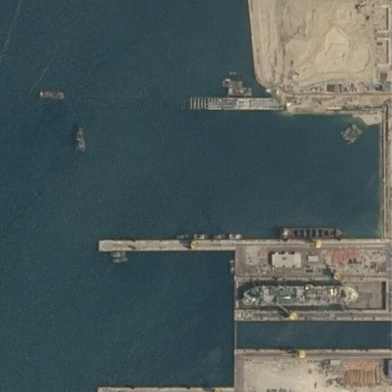
\includegraphics[width=\textwidth]{images/categorical_accuracy_image}
        \caption{Original Image}
        \label{fig:ca_image}
    \end{subfigure}
    \hfill
    \begin{subfigure}{\CategoricalAccuracyImageWidth}
        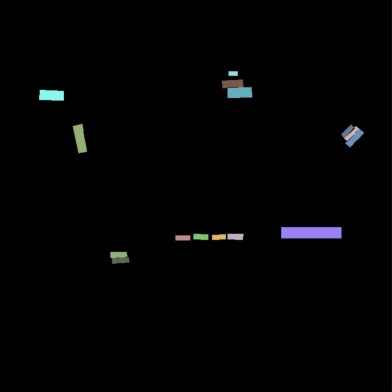
\includegraphics[width=\textwidth]{images/categorical_accuracy_label}
        \caption{Ground Truth}
        \label{fig:ca_truth}
    \end{subfigure}
    \hfill
    \begin{subfigure}{\CategoricalAccuracyImageWidth}
        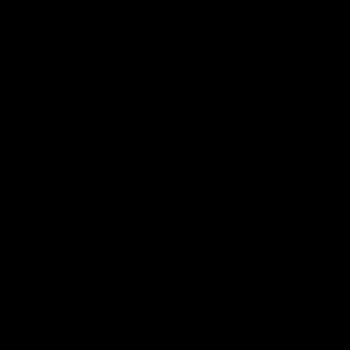
\includegraphics[width=\textwidth]{images/categorical_accuracy_prediction}
        \caption{Model Prediction}
        \label{fig:ca_prediction}
    \end{subfigure}
    \hfill
    \caption[Drawbacks for Categorical Accuracy regarding Dominant Classes]{Drawbacks for Categorical Accuracy regarding Dominant Classes~\cite{tds_segmentation18}}
    \label{fig:categorical_accuracy_drawbacks}
\end{figure}

Although this metric is generally useful for a first impression of performance, it has a major drawback when it comes to class imbalances~\cite{tds_segmentation18}. If there is a dominant class, which takes up a majority of the pixels (like e.~g. a background class), the performance estimation of categorical accuracy can be very misleading. Figure~\ref{fig:categorical_accuracy_drawbacks} demonstrates such a case. The categorical accuracy is computed to be around $95\%$ and seems very promising. But a look at the actual predictions reveals that the model clearly missed the developer's intent. The consequence is, that a high categorical accuracy does not necessarily imply strong segmentation results.

There are some ways to overcome this issue, for example to calculate and check the categorical accuracy for each class separately. This helps to understand which classes the model can predict reliably and which classes causes trouble. In general it is recommended to also integrate other metrics into the evaluation process in order to obtain a wider perspective.

The \emph{intersection over union} (IoU) is another metric which is commonly used to evaluate segmentation results~\cite{pascal_voc15}. It is computed using two values:
\begin{enumerate}
    \item the area of intersection of the prediction with the ground truth, which is equal to the number of correctly predicted pixels
    \item and the area of union of both prediction and ground truth, which includes correct predictions as well as false positives and false negatives.
\end{enumerate}

The IoU is defined as the ratio between those two values (see equation~\ref{eq:mean_iou}). For multi-class challenges, the IoU is computed separately for each class and then averaged over all classes. This is then called \emph{Mean IoU}.

\begin{equation}
    \label{eq:mean_iou}
    \text{IoU} = \frac{\text{true pos.}}{\text{true pos.}+\text{false pos.}+\text{false neg.}}
\end{equation}

Coming back to the example in figure~\ref{fig:categorical_accuracy_drawbacks}, the Mean IoU is at around $47\%$ (assuming $\sim 0\%$ for ships and $\sim 95\%$ for background). While the metric does still not form a perfect indicator for real-world usability of the predictions, it at least directly correlates to segmentation quality. This means a high Mean IoU implies strong segmentation results in most cases.

\subsection{Reference Architectures}
\label{sec:ref_archs}
CNNs play a key role in all computer vision tasks. While a DNN is able to compute a non-linear function, a CNN with a proper architecture allows to compute a non-linear filter. That is the case if the network exclusively consists of layers that operate on the spatial features only (i.~e. no fully-connected layers).

The idea of fully convolutional networks (FCNs) was first introduced by Long et al.\ in~\cite{fcn15}. They took existing CNN architectures like AlexNet~\cite{alexnet12} and transformed them to the FCN concept by replacing all fully-connected layers with $1\times 1$ convolution layers. That way, the spatial nature of the input was preserved and the output basically formed a heatmap highlighting the parts of the input that the prediction was based on. Later on, they used convolution layers with fractional strides as a way to upsample the resolution with trainable filters. Eventually, this led from the coarse heatmaps to class predictions at the pixel level, which is essentially a semantic segmentation.

Since then, many network architectures have been explored. The architecture affects the quality of the network significantly, thus it is important to choose a matching architecture for the question at hand. There is plenty of research going on for architectural patterns that benefit towards semantic segmentation. In this thesis, three well-performing network architectures have been picked to explore their capabilities of carrying out terrain type segmentation. The following subsections will present these architectures in detail.

\subsubsection{U-Net Architecture}
\label{sec:unet}
In 2015, Ronneberger et al.\ introduced an architecture called \emph{U-Net} which they recommended for binary segmentation of biomedical images~\cite{unet15}. It consists of a contracting path in the beginning, in which convolution and pooling layers are used to condense the input. The second half forms an expansive part, that uses convolution and upsampling layers to go back to the scale of the original image (see figure~\ref{fig:unet_architecture}). Note that the outputs of the convolution layers in the contracting path are cropped and then concatenated to the input layers with the corresponding size in the expansive path. These connections between layers that are not directly adjacent to each other are called \emph{skip connections}. By doing that, the expansive layers still retain enough information from the original input to deliver a precise segmentation.

As can be seen in figure~\ref{fig:unet_architecture}, the name U-Net derives from the U-shape of the network model. The input layer expects a $572\times 572$ pixels image with only one feature channel (i.~e. the inputs are grayscale images). The contracting path consists of downsampling blocks with repeated $3\times 3$ unpadded convolutions with ReLU activation followed by a $2\times 2$ max pooling layer. After each downsampling block, the number of feature maps is doubled. In total, there are four downsampling blocks resulting in $32\times 32$ pixels resolution with $1024$ feature maps at the lowest level.

For the expansive path, an upsampling layer followed by a $2\times 2$ convolution layer is used to increase the spatial extents again. At the same time, each upsampling step halves the number of feature maps and then concatenates the cropped feature maps of the corresponding size of the contracting path. After that, two $3\times 3$ unpadded convolutions with ReLU activations are applied to form one upsampling block. In total, there are four upsampling blocks eventually landing at a resolution of $388\times 388$ pixels. Finally, a single $1\times 1$ convolution layer with softmax activation carries out the final segmentation. Therefore, the number of feature maps for this last convolution layer matches the number of classes to predict.

\begin{figure}[h]
    \centering
    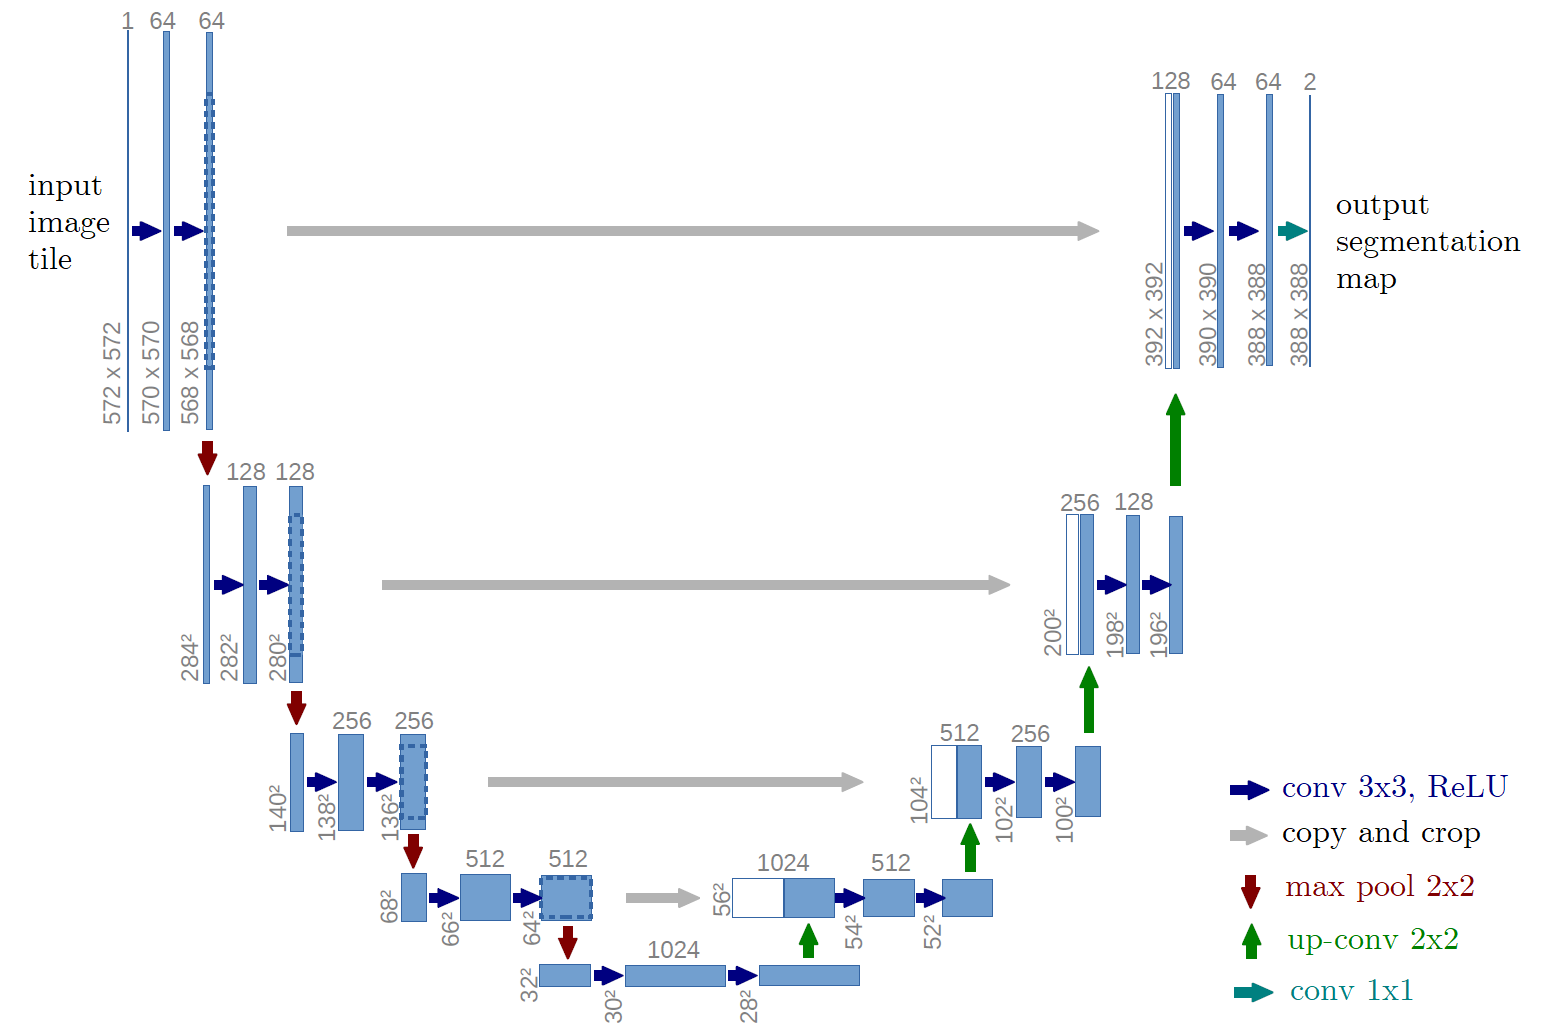
\includegraphics[width=0.8\textwidth]{images/u-net-architecture}
    \caption[U-Net Reference Architecture]{U-Net Reference Architecture~\cite{unet15}}
    \label{fig:unet_architecture}
\end{figure}

The U-Net architecture contains neither fully connected layers nor do they use padding for the edges in the convolution layers. Thus, the edges of the image are being cropped and the resulting segmentation map has a lower resolution than the original image. With that strategy, the edges of the predicted segmentation tend to be more accurate, because they still have all the contextual information (i.~e. their surrounding pixels) available. By using a tiling strategy with overlapping tiles, this approach can produce seamless segmentation maps for input images of arbitrary size. For the edges of the input image, Ronneberger et al.\ suggest a mirroring strategy to extrapolate the missing context~\cite{unet15}.

\subsubsection{DenseNet Architecture}
\label{sec:densenet}
As the depth of CNN architectures tends to increase, a new challenge arose regarding the training of those networks. Since the hidden layers can be very far away from the input and output layers, the values and gradients passed between the layers can get lost on the way. In an attempt to solve this, Huang et al.\ came up with the idea to directly connect all layers with matching feature map sizes. They published their architecture with the name \emph{DenseNet} in~\cite{densenet18}.

Huang et al.\ consider the values passed between layers to be the network's state. To access the state of one of the early layers in the network with a subsequent layer, all the layers in between have to pass the state unchanged, thus creating redundancy. With the DenseNet architecture, the state of all previous layers is explicitly passed to subsequent layers by concatenating the feature maps. This means, the network now differentiates between information that originates from an earlier layer and new information produced in the current layer. It allows to keep the convolution layers narrow (i.~e. the number of feature maps), because each layer only adds information, but never changes information that was previously acquired. This concept leads to having fewer trainable parameters and an improved flow of gradients, which both reduce the effort for training the network~\cite{densenet18}.

\begin{figure}[h]
    \centering
    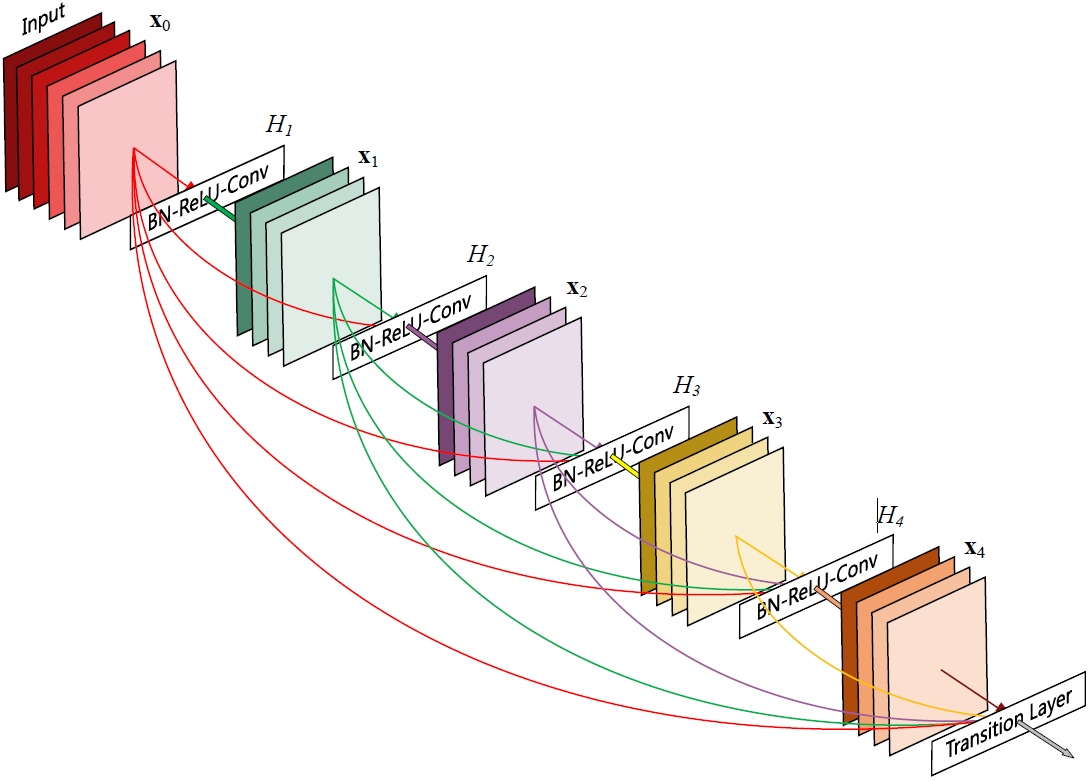
\includegraphics[width=0.7\textwidth]{images/dense-net-architecture}
    \caption[Connections in a 5-layer Dense Block]{Connections in a 5-layer Dense Block~\cite{densenet18}}
    \label{fig:dense_block}
\end{figure}

To still be able to use pooling layers to condense the information in the network, the authors introduce a component called \emph{dense block} (see figure~\ref{fig:dense_block}). Inside of a dense block, they apply dense connections between all subsequent convolution layers. Each square in the figure represents one feature map. The initial input of the dense block consists of six feature maps. Those are passed into a group of batch normalization, ReLU activation and convolution layers (marked with $H_1$ in figure~\ref{fig:dense_block}). The convolution layer produces four new feature maps. The next group of layers ($H_2$) now receives all ten feature maps, again producing four new feature maps. For each group of layers, the number of feature maps increases by four. Huang et al.\ therefore called this factor the \emph{growth rate} of the network.

The overall architecture of DenseNet is made up of multiple dense blocks. In between two consecutive dense blocks, there is a \emph{transition layer}, which is formed by batch normalization, $1\times 1$ convolution and $2\times 2$ average pooling. Since the original DenseNet architecture was designed for the purpose of image classification, the conclusion of the network is a $7\times 7$ global average pooling layer and eventually a fully-connected layer with softmax activation. Thus, the original architecture is incapable of performing semantic segmentation.

However, it is possible to extend the architecture with an upsampling path at the end. By doing that, DenseNets can also be used to enact on segmentation tasks. This approach was first investigated by Jégou et al.~\cite{denseseg17}. Their overall architecture looks very similar to the U-Net architecture (see figure~\ref{fig:densenet_segmentation}). But instead of using standalone convolution layers, the authors used the dense blocks proposed in~\cite{densenet18}. This results in a very densely connected architecture, because now there are connections between all convolution layers as well as the skip connections between the downsampling and upsampling path.

\begin{figure}[h]
    \centering
    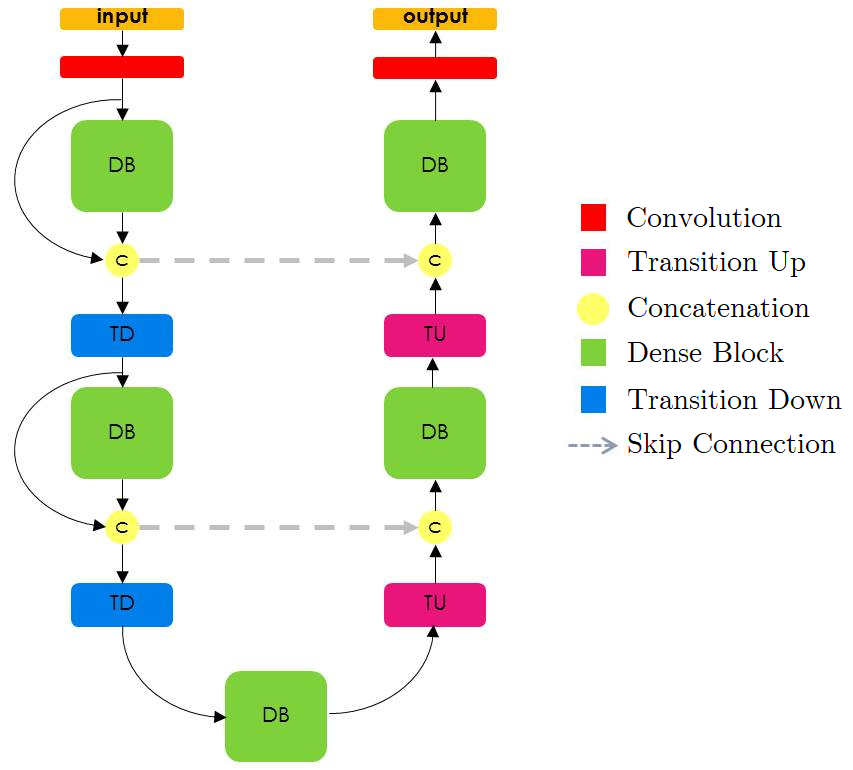
\includegraphics[width=0.65\textwidth]{images/dense_segmentation_architecture}
    \caption[FC-DenseNet Reference Architecture]{FC-DenseNet Reference Architecture~\cite{denseseg17}}
    \label{fig:densenet_segmentation}
\end{figure}

For this architecture, there are two types of transition layers. The \emph{transition down} layer is used for the downsampling path and has the same setup as the transition layer in the original DenseNet. On the other hand, there is a \emph{transition up} layer, which is used in the upsampling path. It consists of a $3\times 3$ transposed convolution with a stride of $2\times 2$. Thus, a transition up layer doubles the spatial extents of the feature maps.

In~\cite{denseseg17}, Jégou et al.\ proposed a configuration for the DenseNet consisting of five dense blocks each followed by transition down as downsampling path, one intermediate dense block to act as a bottleneck layer, and again five dense blocks each followed by transition up as upsampling path. The final layer is a $1\times 1$ convolution layer with softmax activation and $k$ (the number of classes) feature maps. In total, this network contains 103 convolution layers. Because this architecture now only consists of convolution layers, the authors named it \emph{fully convolutional DenseNet} (FC-DenseNet).

\subsubsection{W-Net}
\label{sec:w-net}
Both U-Net and DenseNet architectures are based on the idea of supervised learning. There are also some architectures that approach the image segmentation task with unsupervised learning. The \emph{W-Net} architecture presented in~\cite{wnet17} is one example.

In general, the W-Net architecture consists of two major parts. The first part generates a $k$-class segmentation of the input image. Subsequently, the second part reconstructs the original image only from the segmentation. The loss function then calculates the deviation between the reconstructed and the original image, i.~e. no labels are required. Because of that, the network detects all segmentation classes on its own by clustering the pixels into similar groups. The downside is, that the chosen classes may be completely unrelated to the challenge which is to be solved.

Figure~\ref{fig:wnet_architecture} illustrates the W-Net architecture. The network is split into an encoder part $U_{Enc}$ and a decoder part $U_{Dec}$. The parts themselves are very much based on the U-Net architecture introduced in section~\ref{sec:unet}. Each part has its own contracting path followed by an expansive path with skip connections between layers with matching spatial extents.

\begin{figure}[h]
    \centering
    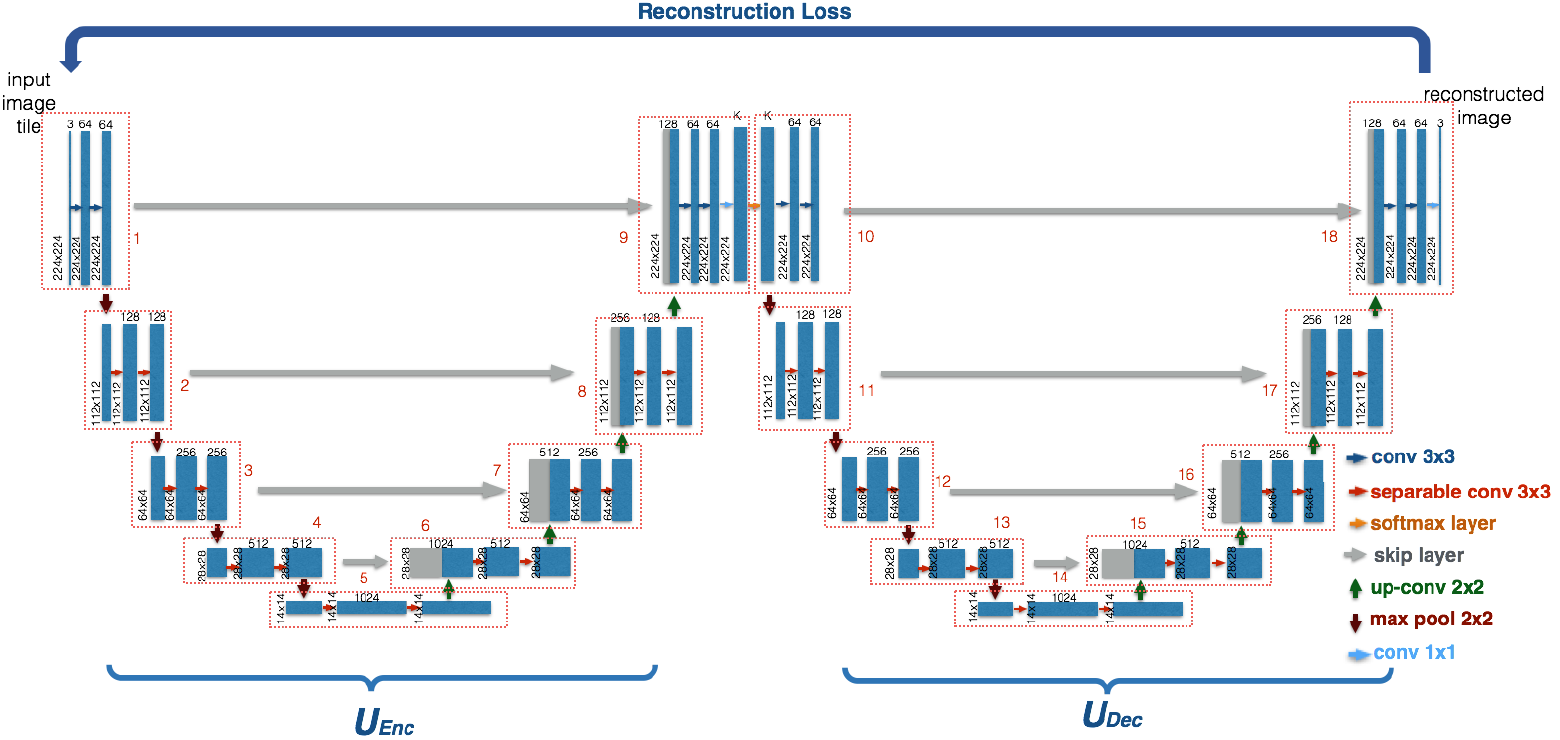
\includegraphics[width=0.95\textwidth]{images/w-net-architecture}
    \caption[W-Net Reference Architecture]{W-Net Reference Architecture~\cite{wnet17}}
    \label{fig:wnet_architecture}
\end{figure}

The last layer of the encoder part is a $1\times 1$ convolution layer. The number of feature maps in this layer (denoted with $K$ in figure~\ref{fig:wnet_architecture}) represents the number of classes to use for the segmentation. The output of the encoder is a one hot encoded vector with the likelihood for each pixel to belong to a certain class. During training, this vector serves as input for the decoder part of the network. The last layer of the decoder is also a $1\times 1$ convolution layer. This layer always consists of three feature maps to restore the color bands of the original image.

As one important difference to the initial U-Net architecture, W-Net uses depthwise separable convolution layers~\cite{depthwise_conv17} in some places instead of regular convolution layers. Regular convolution applies the convolution filters to both the spatial dimensions and the depth dimension (i.~e. the channels of the image) at the same time. In depthwise separable convolution, those two steps are performed separately. The first set of convolution filters is applied to each feature channel separately. Thus, these filters do not change the depth of the image. After that, $n$ filters of size $1\times 1\times c$ are used to condense all $c$ feature channels into a single channel each, resulting in $n$ feature maps in total. By doing that, the network differentiates between spatial correlations and cross-channel correlations independently. This increases the computational efficiency of the model without any significant impact on the effectiveness.

Xia and Kulis propose to follow up the initial segmentation of W-Net with two postprocessing steps~\cite{wnet17}. First, they foster sharp edges for object boundaries by using conditional random fields~\cite{crf17}. In the second step, they reduce over-segmentation of the image by merging segments according to weighted boundary maps~\cite{hierarchy_imgseg11}.

\subsection{Architecture Comparison}
Overall, all of the discussed reference architectures follow the \emph{encoder-decoder} architectural pattern. In the encoder, the number of feature maps is increased while the spatial dimensions are reduced. In a symmetrical fashion, the decoder decreases the number of feature maps while increasing the spatial dimensions. This is a very common pattern that is used by many image segmentation architectures~\cite{imseg_survey20}. It enables to capture enough context for each pixel and still provides precise localization.

It is difficult to compare the actual performance of the three architectures, since they were all trained and evaluated on different datasets with differing metrics. However, some metrics are reviewed considering the context and complexity of their particular challenge. Additionally, figure~\ref{fig:segmentation_examples} provides visual examples of the segmentation results of the three different approaches.

\begin{figure}
    \newcommand{\SegmentationExampleImageWidth}{0.3\textwidth}
    \centering
    \hfill
    \begin{subfigure}{\SegmentationExampleImageWidth}
        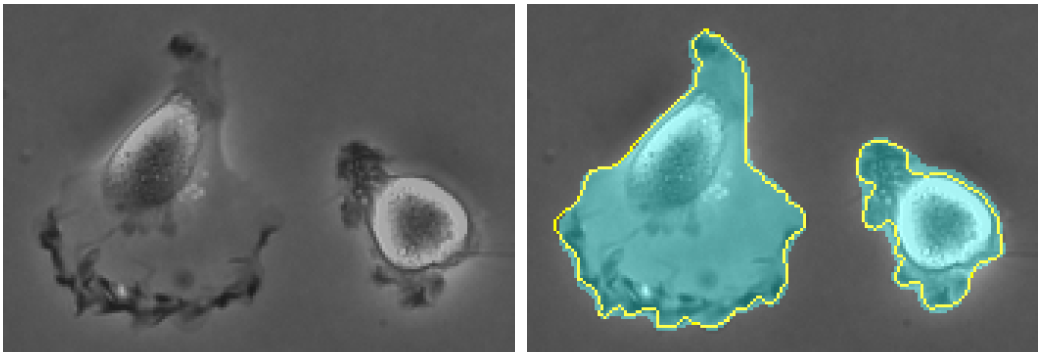
\includegraphics[width=\textwidth]{images/segmentation_example_unet}
        \caption{U-Net~\cite{unet15}}
        \label{fig:exseg_unet}
    \end{subfigure}
    \hfill
    \begin{subfigure}{0.4\textwidth}
        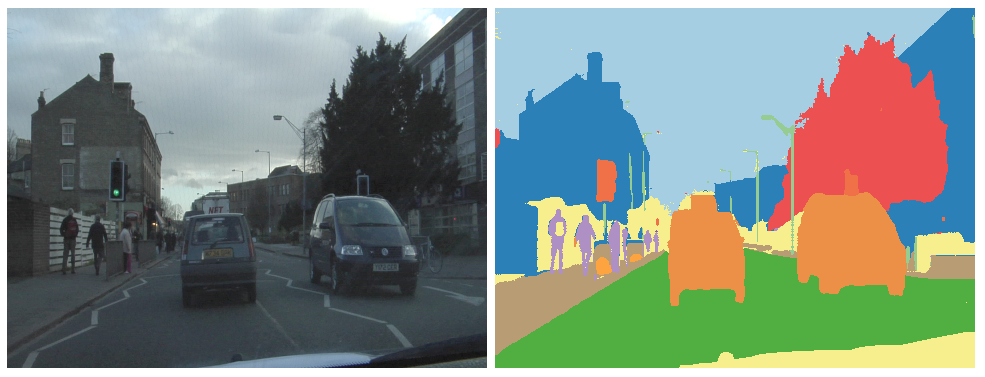
\includegraphics[width=\textwidth]{images/segmentation_example_densenet}
        \caption{DenseNet~\cite{denseseg17}}
        \label{fig:exseg_densenet}
    \end{subfigure}
    \hfill
    \begin{subfigure}{0.21\textwidth}
        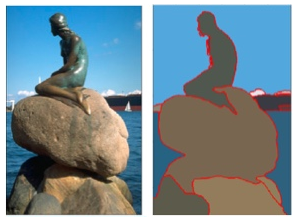
\includegraphics[width=\textwidth]{images/segmentation_example_wnet}
        \caption{W-Net~\cite{wnet17}}
        \label{fig:exseg_wnet}
    \end{subfigure}
    \hfill
    \caption{Segmentation Results from the Reference Architectures}
    \label{fig:segmentation_examples}
\end{figure}

U-Net was trained and evaluated for the ISBI cell tracking challenge~\cite{isbi_challenge12}. The challenge consists of two datasets, both showing biological cells scanned with different microscopy techniques. For both datasets the main objective was to provide a binary classification for the cell images, where a distinction between cell and non-cell pixels must be made. Also the precise detection of boundaries between adjacent cells was a key point of interest for this challenge. The U-Net model with around $31$ million parameters achieved an average IoU of $92.03\%$ for the PhC-U373 and $77.56\%$ for the DIC-HeLa datasets~\cite{unet15}. One example segmentation for the DIC-HeLa dataset is shown in Figure~\ref{fig:exseg_unet}.

To train and evaluate the FC-DenseNet the CamVid dataset~\cite{camvid_challenge} was used. CamVid is a database of urban scene videos, fully labelled with 32 different classes. The classes include moving objects like pedestrians and cars, ceilings like sky and tunnel as well as fixed objects like buildings, roads and fences. The authors of FC-DenseNet report a mean IoU of $66.9\%$ and a global accuracy of $91.5\%$~\cite{denseseg17}. Only looking at the plain numbers, FC-DenseNet seems worse than U-Net because of the lower mean IoU. However, with only around $9.4$ million parameters it requires significantly less computational power. Also, the CamVid dataset is much more sophisticated compared to the ISBI cell tracking challenge. As can be seen in figure~\ref{fig:exseg_densenet}, the segmentation predictions of FC-DenseNet are of high quality.

W-Net was trained on the PASCAL VOC 2012 dataset~\cite{pascal_voc12} and evaluated with the Berkeley Segmentation Database (BSDS500)~\cite{hierarchy_imgseg11}. Both datasets contain hundreds of images with precisely labelled segmentation maps. But since the W-Net architecture is trained in an unsupervised approach, the labels of the datasets are only used for evaluation. Also, the performance metrics are different, because there are multiple ground-truth labels for each image in the dataset. For example, they use a metric called \emph{segmentation covering}~(SC)~\cite{hierarchy_imgseg11}, which is an extension to the well-known IoU metric.

Without postprocessing, W-Net scores $62\%$ SC on the BSDS500 dataset. Again, according to the plain numbers this seems worse than the results of U-Net and DenseNet. But taking into account, that W-Net was trained with unsupervised learning, i.~e. it did not receive any labelling information during training, the results are quite remarkable. Figure~\ref{fig:exseg_wnet} presents a segmentation map predicted by W-Net.

Overall, it is difficult to judge which architecture has delivered the best results in general. Likewise, it is not possible to draw conclusions about which architecture works best on the given problem of terrain type segmentation. Therefore in section~\ref{sec:segmentation} all three architectures are implemented and evaluated for this specific task.

\clearpage